\documentclass[journal, monochrome]{IEEEtran}
\usepackage[utf8]{inputenc}
\usepackage[monochrome]{color}
\usepackage{graphicx}
\usepackage{amsmath}
\usepackage{amssymb}
\usepackage{fancyvrb}
\usepackage{dsfont}
\usepackage{subfigure}
\usepackage{natbib}
\usepackage{moreverb}
\usepackage{url}
\usepackage{listings}
\usepackage{courier}
\usepackage{caption}

\lstloadlanguages{Octave}
\captionsetup[lstlisting]{ singlelinecheck=false, margin=0pt, font={bf,footnotesize}}
\lstset{
  basicstyle=\footnotesize\ttfamily,
  %numbers=left,
  numberstyle=\tiny,
  %stepnumber=2,
  numbersep=5pt,
  tabsize=8,
  extendedchars=true,
  breaklines=true,
  framexleftmargin=17pt,
  framexrightmargin=5pt,
  showstringspaces=false
}

\ifCLASSINFOpdf
\else
\fi
% graphicx was written by David Carlisle and Sebastian Rahtz. It is
% required if you want graphics, photos, etc. graphicx.sty is already
% installed on most LaTeX systems. The latest version and documentation can
% be obtained at: 
% http://www.ctan.org/tex-archive/macros/latex/required/graphics/
% Another good source of documentation is "Using Imported Graphics in
% LaTeX2e" by Keith Reckdahl which can be found as epslatex.ps or
% epslatex.pdf at: http://www.ctan.org/tex-archive/info/
%
% latex, and pdflatex in dvi mode, support graphics in encapsulated
% postscript (.eps) format. pdflatex in pdf mode supports graphics
% in .pdf, .jpeg, .png and .mps (metapost) formats. Users should ensure
% that all non-photo figures use a vector format (.eps, .pdf, .mps) and
% not a bitmapped formats (.jpeg, .png). IEEE frowns on bitmapped formats
% which can result in "jaggedy"/blurry rendering of lines and letters as
% well as large increases in file sizes.
%
% You can find documentation about the pdfTeX application at:
% http://www.tug.org/applications/pdftex





% *** MATH PACKAGES ***
%
%\usepackage[cmex10]{amsmath}
% A popular package from the American Mathematical Society that provides
% many useful and powerful commands for dealing with mathematics. If using
% it, be sure to load this package with the cmex10 option to ensure that
% only type 1 fonts will utilized at all point sizes. Without this option,
% it is possible that some math symbols, particularly those within
% footnotes, will be rendered in bitmap form which will result in a
% document that can not be IEEE Xplore compliant!
%
% Also, note that the amsmath package sets \interdisplaylinepenalty to 10000
% thus preventing page breaks from occurring within multiline equations. Use:
%\interdisplaylinepenalty=2500
% after loading amsmath to restore such page breaks as IEEEtran.cls normally
% does. amsmath.sty is already installed on most LaTeX systems. The latest
% version and documentation can be obtained at:
% http://www.ctan.org/tex-archive/macros/latex/required/amslatex/math/





% *** SPECIALIZED LIST PACKAGES ***
%
%\usepackage{algorithmic}
% algorithmic.sty was written by Peter Williams and Rogerio Brito.
% This package provides an algorithmic environment fo describing algorithms.
% You can use the algorithmic environment in-text or within a figure
% environment to provide for a floating algorithm. Do NOT use the algorithm
% floating environment provided by algorithm.sty (by the same authors) or
% algorithm2e.sty (by Christophe Fiorio) as IEEE does not use dedicated
% algorithm float types and packages that provide these will not provide
% correct IEEE style captions. The latest version and documentation of
% algorithmic.sty can be obtained at:
% http://www.ctan.org/tex-archive/macros/latex/contrib/algorithms/
% There is also a support site at:
% http://algorithms.berlios.de/index.html
% Also of interest may be the (relatively newer and more customizable)
% algorithmicx.sty package by Szasz Janos:
% http://www.ctan.org/tex-archive/macros/latex/contrib/algorithmicx/




% *** ALIGNMENT PACKAGES ***
%
%\usepackage{array}
% Frank Mittelbach's and David Carlisle's array.sty patches and improves
% the standard LaTeX2e array and tabular environments to provide better
% appearance and additional user controls. As the default LaTeX2e table
% generation code is lacking to the point of almost being broken with
% respect to the quality of the end results, all users are strongly
% advised to use an enhanced (at the very least that provided by array.sty)
% set of table tools. array.sty is already installed on most systems. The
% latest version and documentation can be obtained at:
% http://www.ctan.org/tex-archive/macros/latex/required/tools/


%\usepackage{mdwmath}
%\usepackage{mdwtab}
% Also highly recommended is Mark Wooding's extremely powerful MDW tools,
% especially mdwmath.sty and mdwtab.sty which are used to format equations
% and tables, respectively. The MDWtools set is already installed on most
% LaTeX systems. The lastest version and documentation is available at:
% http://www.ctan.org/tex-archive/macros/latex/contrib/mdwtools/


% IEEEtran contains the IEEEeqnarray family of commands that can be used to
% generate multiline equations as well as matrices, tables, etc., of high
% quality.


%\usepackage{eqparbox}
% Also of notable interest is Scott Pakin's eqparbox package for creating
% (automatically sized) equal width boxes - aka "natural width parboxes".
% Available at:
% http://www.ctan.org/tex-archive/macros/latex/contrib/eqparbox/





% *** SUBFIGURE PACKAGES ***
%\usepackage[tight,footnotesize]{subfigure}
% subfigure.sty was written by Steven Douglas Cochran. This package makes it
% easy to put subfigures in your figures. e.g., "Figure 1a and 1b". For IEEE
% work, it is a good idea to load it with the tight package option to reduce
% the amount of white space around the subfigures. subfigure.sty is already
% installed on most LaTeX systems. The latest version and documentation can
% be obtained at:
% http://www.ctan.org/tex-archive/obsolete/macros/latex/contrib/subfigure/
% subfigure.sty has been superceeded by subfig.sty.



%\usepackage[caption=false]{caption}
%\usepackage[font=footnotesize]{subfig}
% subfig.sty, also written by Steven Douglas Cochran, is the modern
% replacement for subfigure.sty. However, subfig.sty requires and
% automatically loads Axel Sommerfeldt's caption.sty which will override
% IEEEtran.cls handling of captions and this will result in nonIEEE style
% figure/table captions. To prevent this problem, be sure and preload
% caption.sty with its "caption=false" package option. This is will preserve
% IEEEtran.cls handing of captions. Version 1.3 (2005/06/28) and later 
% (recommended due to many improvements over 1.2) of subfig.sty supports
% the caption=false option directly:
%\usepackage[caption=false,font=footnotesize]{subfig}
%
% The latest version and documentation can be obtained at:
% http://www.ctan.org/tex-archive/macros/latex/contrib/subfig/
% The latest version and documentation of caption.sty can be obtained at:
% http://www.ctan.org/tex-archive/macros/latex/contrib/caption/




% *** FLOAT PACKAGES ***
%
%\usepackage{fixltx2e}
% fixltx2e, the successor to the earlier fix2col.sty, was written by
% Frank Mittelbach and David Carlisle. This package corrects a few problems
% in the LaTeX2e kernel, the most notable of which is that in current
% LaTeX2e releases, the ordering of single and double column floats is not
% guaranteed to be preserved. Thus, an unpatched LaTeX2e can allow a
% single column figure to be placed prior to an earlier double column
% figure. The latest version and documentation can be found at:
% http://www.ctan.org/tex-archive/macros/latex/base/



%\usepackage{stfloats}
% stfloats.sty was written by Sigitas Tolusis. This package gives LaTeX2e
% the ability to do double column floats at the bottom of the page as well
% as the top. (e.g., "\begin{figure*}[!b]" is not normally possible in
% LaTeX2e). It also provides a command:
%\fnbelowfloat
% to enable the placement of footnotes below bottom floats (the standard
% LaTeX2e kernel puts them above bottom floats). This is an invasive package
% which rewrites many portions of the LaTeX2e float routines. It may not work
% with other packages that modify the LaTeX2e float routines. The latest
% version and documentation can be obtained at:
% http://www.ctan.org/tex-archive/macros/latex/contrib/sttools/
% Documentation is contained in the stfloats.sty comments as well as in the
% presfull.pdf file. Do not use the stfloats baselinefloat ability as IEEE
% does not allow \baselineskip to stretch. Authors submitting work to the
% IEEE should note that IEEE rarely uses double column equations and
% that authors should try to avoid such use. Do not be tempted to use the
% cuted.sty or midfloat.sty packages (also by Sigitas Tolusis) as IEEE does
% not format its papers in such ways.


%\ifCLASSOPTIONcaptionsoff
%  \usepackage[nomarkers]{endfloat}
% \let\MYoriglatexcaption\caption
% \renewcommand{\caption}[2][\relax]{\MYoriglatexcaption[#2]{#2}}
%\fi
% endfloat.sty was written by James Darrell McCauley and Jeff Goldberg.
% This package may be useful when used in conjunction with IEEEtran.cls'
% captionsoff option. Some IEEE journals/societies require that submissions
% have lists of figures/tables at the end of the paper and that
% figures/tables without any captions are placed on a page by themselves at
% the end of the document. If needed, the draftcls IEEEtran class option or
% \CLASSINPUTbaselinestretch interface can be used to increase the line
% spacing as well. Be sure and use the nomarkers option of endfloat to
% prevent endfloat from "marking" where the figures would have been placed
% in the text. The two hack lines of code above are a slight modification of
% that suggested by in the endfloat docs (section 8.3.1) to ensure that
% the full captions always appear in the list of figures/tables - even if
% the user used the short optional argument of \caption[]{}.
% IEEE papers do not typically make use of \caption[]'s optional argument,
% so this should not be an issue. A similar trick can be used to disable
% captions of packages such as subfig.sty that lack options to turn off
% the subcaptions:
% For subfig.sty:
% \let\MYorigsubfloat\subfloat
% \renewcommand{\subfloat}[2][\relax]{\MYorigsubfloat[]{#2}}
% For subfigure.sty:
% \let\MYorigsubfigure\subfigure
% \renewcommand{\subfigure}[2][\relax]{\MYorigsubfigure[]{#2}}
% However, the above trick will not work if both optional arguments of
% the \subfloat/subfig command are used. Furthermore, there needs to be a
% description of each subfigure *somewhere* and endfloat does not add
% subfigure captions to its list of figures. Thus, the best approach is to
% avoid the use of subfigure captions (many IEEE journals avoid them anyway)
% and instead reference/explain all the subfigures within the main caption.
% The latest version of endfloat.sty and its documentation can obtained at:
% http://www.ctan.org/tex-archive/macros/latex/contrib/endfloat/
%
% The IEEEtran \ifCLASSOPTIONcaptionsoff conditional can also be used
% later in the document, say, to conditionally put the References on a 
% page by themselves.





% *** PDF, URL AND HYPERLINK PACKAGES ***
%
%\usepackage{url}
% url.sty was written by Donald Arseneau. It provides better support for
% handling and breaking URLs. url.sty is already installed on most LaTeX
% systems. The latest version can be obtained at:
% http://www.ctan.org/tex-archive/macros/latex/contrib/misc/
% Read the url.sty source comments for usage information. Basically,
% \url{my_url_here}.





% *** Do not adjust lengths that control margins, column widths, etc. ***
% *** Do not use packages that alter fonts (such as pslatex).         ***
% There should be no need to do such things with IEEEtran.cls V1.6 and later.
% (Unless specifically asked to do so by the journal or conference you plan
% to submit to, of course. )


% correct bad hyphenation here
\hyphenation{op-tical net-works semi-conduc-tor}


\begin{document}
%
% paper title
% can use linebreaks \\ within to get better formatting as desired
\title{Análisis de la velocidad del viento en Irlanda}
%
%
% author names and IEEE memberships
% note positions of commas and nonbreaking spaces ( ~ ) LaTeX will not break
% a structure at a ~ so this keeps an author's name from being broken across
% two lines.
% use \thanks{} to gain access to the first footnote area
% a separate \thanks must be used for each paragraph as LaTeX2e's \thanks
% was not built to handle multiple paragraphs
%

\author{\textbf{Autores:} Alejandro Magnorsky, Andrés Mata Suárez, Mariano Merchante \\[5px]
        Instituto Tecnológico de Buenos Aires}
        
% note the % following the last \IEEEmembership and also \thanks - 
% these prevent an unwanted space from occurring between the last author name
% and the end of the author line. i.e., if you had this:
% 
% \author{....lastname \thanks{...} \thanks{...} }
%                     ^------------^------------^----Do not want these spaces!
%
% a space would be appended to the last name and could cause every name on that
% line to be shifted left slightly. This is one of those "LaTeX things". For
% instance, "\textbf{A} \textbf{B}" will typeset as "A B" not "AB". To get
% "AB" then you have to do: "\textbf{A}\textbf{B}"
% \thanks is no different in this regard, so shield the last } of each \thanks
% that ends a line with a % and do not let a space in before the next \thanks.
% Spaces after \IEEEmembership other than the last one are OK (and needed) as
% you are supposed to have spaces between the names. For what it is worth,
% this is a minor point as most people would not even notice if the said evil
% space somehow managed to creep in.



% The paper headers
%\markboth{Template para los informes de SS, 2011}
%{Shell \MakeLowercase{\textit{et al.}}: Bare Demo of IEEEtran.cls for Journals}
% The only time the second header will appear is for the odd numbered pages
% after the title page when using the twoside option.
% 
% *** Note that you probably will NOT want to include the author's ***
% *** name in the headers of peer review papers.                   ***
% You can use \ifCLASSOPTIONpeerreview for conditional compilation here if
% you desire.




% If you want to put a publisher's ID mark on the page you can do it like
% this:
%\IEEEpubid{0000--0000/00\$00.00~\copyright~2007 IEEE}
% Remember, if you use this you must call \IEEEpubidadjcol in the second
% column for its text to clear the IEEEpubid mark.



% use for special paper notices
%\IEEEspecialpapernotice{(Invited Paper)}












% make the title area
\maketitle

\renewcommand{\abstractname}{Resumen}
\renewcommand{\IEEEkeywordsname}{Palabras clave}
\renewcommand{\refname}{Referencias}
\renewcommand{\tablename}{Tabla}

\begin{abstract}
\boldmath

\end{abstract}
% IEEEtran.cls defaults to using nonbold math in the Abstract.
% This preserves the distinction between vectors and scalars. However,
% if the journal you are submitting to favors bold math in the abstract,
% then you can use LaTeX's standard command \boldmath at the very start
% of the abstract to achieve this. Many IEEE journals frown on math
% in the abstract anyway.

% Note that keywords are not normally used for peerreview papers.
\begin{IEEEkeywords}
Velocidad del viento; Cuadrados mínimos; Irlanda.
\end{IEEEkeywords}






% For peer review papers, you can put extra information on the cover
% page as needed:
% \ifCLASSOPTIONpeerreview
% \begin{center} \bfseries EDICS Category: 3-BBND \end{center}
% \fi
%
% For peerreview papers, this IEEEtran command inserts a page break and
% creates the second title. It will be ignored for other modes.
\IEEEpeerreviewmaketitle
\vspace{1cm}

\section{Introducción}
\par
La energía eólica es aquella obtenida a partir del viento. Se trata de energía cinética generada por medio de las corrientes de aire, la cual es transformada en otras formas útiles de energía para las actividades humanas. Las ventajas de la energía eólica es que es un recurso abundante, renovable y limpio. Sin embargo, el principal inconveniente es su intermitencia. 
\par
Para poder aprovechar la energía eólica es importante conocer la velocidad del viento. Esto incluye la velocidad máxima y mínima. Para poder utilizar la energía del viento, es necesario que éste alcance una velocidad mínima que depende del aerogenerador que se vaya a utilizar pero que suele empezar entre los 3 m/s y los 4 m/s, sin exceder los 25 m/s. En los aerogeneradores la energía eólica mueve una hélice y mediante un sistema mecánico se hace girar el rotor de un generador que produce energía eléctrica. Para que su instalación resulte rentable, suelen agruparse en concentraciones denominadas parques eólicos.
\par
El gobierno irlandés consideró la posibilidad de utilizar la energía eólica para satisfacer una porción significativa de las necesidades energéticas de Irlanda. Para determinar la conveniencia y los lugares con mayor potencial se realizó un relevamiento de las velocidades del viento medidas por 12 estaciones meteorológicas
distribuidas a lo largo del territorio. Cabe mencionar que existen distintas escalas de implementación de energía eólica: desde la calefacción de edificios hasta el abastecimiento de energía eléctrica de un cierto porcentaje de la población de una ciudad. 
\par
Antes de instalar y comenzar a operar un aerogenerador en un potencial lugar para producir otras fuentes de energía usando la eólica se suele utilizar registros de las velocidades del viento en dicha zona a lo largo de varios meses. La energía que puede producir un aerogenerador es una función no lineal de la velocidad del viento. Por lo tanto, el cálculo de la velocidad media del viento en la zona es insuficiente. Se hace, entonces, necesaria la estimación de la distribución completa de las velocidades \citep{haslett}.
\par
En la sección \ref{section:development} se calcula el promedio de las velocidades de los vientos para cada estacion meteorológica y se ajustan los datos de las velocidades a una función usando cuadrados mínimos.
\vspace{1cm}
%-------------------------------------------------------------------------
\section{Desarrollo}
\label{section:development}

\subsection{Velocidades medias}
\par
Con el fin de conocer mejor cómo son los datos obtenidos de la medición de la velocidad del viento en las distintas estaciones, se calcula el promedio de todos los datos en cada una de ellas. El resultado de ello se encuentra en la tabla \ref{table:speed}.

\begin{table}
	\begin{center}
		\begin{tabular}{l|r}
			Estación meteorológica & Velocidad media (m/s) \\
			\hline
			Roche's Pt. & 6.3604 \\ 
			Valentia & 5.4770 \\
			Rosslare & 5.9984 \\
			Kilkenny & 3.2442 \\
			Shannon & 5.3794 \\
			Birr & 3.6485 \\
			Dublin & 5.0399 \\
			Claremorris & 4.3699 \\
			Mullingar & 4.3706 \\
			Clones & 4.4794 \\
			Belmullet & 6.7500 \\
			Malin head & 8.0250 \\
		\end{tabular}
		\caption{Velocidades medias en cada estación meteorológica.}
		\label{table:speed}
	\end{center}
\end{table}

\vspace{0.5cm}


\subsection{Aproximación de los datos a una función}
\par
Para cada una de las estaciones meteorológicas, se desea ajustar las velocidades medidas a una función de la forma:
\begin{equation}
v(t) = A_{0} + A_{1}cos(2\pi f_{1}t) + B_{1}sen(2\pi f_{1}t)
\label{equation:model}
\end{equation}
donde $t$ es el tiempo en días, $v(t)$ es la velocidad del viento en el instante $t$ y $f_{1} = \frac{1}{365,25} dia^{-1}$. \\
$v(t)$ es lineal en función de $A_{0}$, $A_{1}$ y $B_{1}$ y se puede expresar como $v(t) = A_{0}f_{1}(t) + A_{1}f_{2}(t) + B_{1}f_{3}(t)$ donde $f_{1}(t) = 1$, $f_{2}(t) = cos(2\pi f_{1}t)$ y $f_{3}(t) = sen(2\pi f_{1}t)$.
\par
Para resolver el problema de ajuste se utiliza el método de cuadrados mínimos \citep{mathews}. El objetivo entonces es encontrar $A_{0}$, $A_{1}$ y $B_{1}$ tal que 
$\displaystyle\sum_{\substack{k=1}}^{n} (v_{k} - v(t_{k}))^{2} $ sea mínimo.
\par
Si definimos la matriz A y los vectores $\vec{x}$ y $\vec{b}$ como:
\begin{equation}
A = \left(\begin{array}{ccc}
f_{1}(t_{1}) & f_{2}(t_{1}) & f_{3}(t_{1}) \\
f_{1}(t_{2}) & f_{2}(t_{2}) & f_{3}(t_{2}) \\
\vdots & \vdots & \vdots \\
f_{1}(t_{n}) & f_{2}(t_{n}) & f_{3}(t_{n}) \\
\end{array} \right) \qquad
\vec{x} = \left(\begin{array}{c}
A_{0} \\
A_{1} \\
B_{1} \\
\end{array} \right) \qquad
\vec{b} = \left(\begin{array}{c}
v_{1} \\
v_{2} \\
\vdots \\
v_{n} \\
\end{array} \right)
\end{equation}
entonces, el objetivo puede expresarse como encontrar $\vec{x}$ tal que $||A\vec{x} - {b}||^{2}$ sea mínimo.
\par
La solución clásica al problema de cuadrados mínimos es hacer $\vec{x} = (A^{T}A)^{-1}A^{T}\vec{b}$. Sin embargo, calcular la inversa de una matriz es de $O(n^{3})$. Es por eso que se optó por resolver el problema utilizando la factorización QR obtenida por:
\begin{itemize}
\item Householder
\item Givens
\item Gram-Schmidt
\end{itemize}
\par
La forma de resolver el problema de cuadrados mínimos usando QR consiste en:
\begin{equation}
A = QR = (Q_{1} \, Q_{2}) \left( \begin{array}{c}
R_{1} \\
0 \\
\end{array} \right)
\end{equation}
donde A tiene dimensiones $n$x$3$, $Q_{1}$ de $n$x$3$, $Q_{2}$ de $n$x$(n-3)$ y $R_{1}$ de $3$x$3$.
\par
La solución se obtiene resolviendo $R_{1}\vec{x} = Q_{1}^{T}\vec{b} $ por sustitución hacia atrás ya que $R_{1}$ es triangular superior.

\subsection{Cálculo del error cuadrático medio de la aproximación}
\par
El error cuadrático medio se calcula mediante la siguiente ecuación:
\begin{equation}
 E_{cm} = \sqrt{\frac{\sum_{k=1}^n e_k^2}{n}} = \sqrt{\frac{||Q_{2}^{T}\vec{b}||^{2}}{n}}
\end{equation}
siendo $e_k$ el error en un punto $(t_k, v_k)$, tal que:
\begin{equation}
 e_k = v_k - v(t_k)
\end{equation}
para un conjunto de $n$ mediciones de la velocidad el viento $v_k$ para el día número $t_k$.\\

!!!!!!!! MEJORAR GIVENS USANDO LA FORMA DE LAS MATRICES G

\begin{table}
	\begin{center}
		\begin{tabular}{l|r}
			Estación meteorológica & $E_{cm}$ (m/s) \\
			\hline
			Roche's Pt. & 2.7777 \\ 
			Valentia & 2.6051 \\
			Rosslare & 2.4946 \\
			Kilkenny & 1.8217 \\
			Shannon & 2.4984 \\
			Birr & 2.0097 \\
			Dublin & 2.4404 \\
			Claremorris & 2.2754 \\
			Mullingar & 2.1014 \\
			Clones & 2.2598 \\
			Belmullet & 2.9600 \\
			Malin head & 3.2619 \\
		\end{tabular}
		\caption{Error cuadrático medio para cada estación meteorológica.}
		\label{table:ecm}
	\end{center}
\end{table}

\vspace{0.5cm}
\par
La tabla \ref{table:ecm} muestra los resultados del cálculo del error cuadrático medio para cada estación meteorológica considerada.

\subsection{Valor medio de días por año}

\subsection{Histograma del error}
\begin{figure}[h]
	\begin{center}
		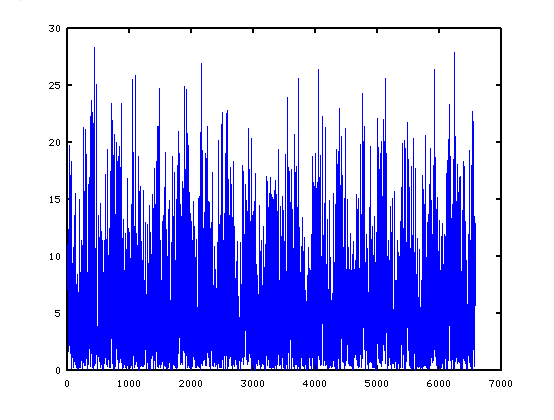
\includegraphics[scale = 0.5]{img/histo.png}
		\caption{Histograma del error}
		\label{figure:histo}
	\end{center}
\end{figure}

\vspace{1cm}
%-------------------------------------------------------------------------
\section{Resultados y conclusiones}
\label{section:results}



\vspace{1cm}
%-------------------------------------------------------------------------

\begin{thebibliography}{1}

\bibitem[Haslett, J. y Raftery, A. E.(1989)]{haslett}
	Haslett, J.,
	Raftery, Adrian E.,
	``Space-time Modelling with
   	Long-memory Dependence: Assessing Ireland's Wind Power Resource'',
	1989 

\bibitem[Mathews y Fink(1992)]{mathews}
	Mathews, John H.,
	Fink, Kurtis D.,
	``Numerical Methods Using MATLAB'',
	Prentice Hall,
	1999
	
\end{thebibliography}

%-------------------------------------------------------------------------


\begin{figure}
	\lstinputlisting[label=lst:householder,caption=Implementación de la factorización QR usando reflexiones de Householder.]{../src/householder.m}
\end{figure}

\begin{figure}
	\lstinputlisting[label=lst:gramschmidt,caption=Implementación de la factorización QR por medio del método de Gram-Schmidt.]{../src/gramSchmidt.m}
\end{figure}

\begin{figure}
	\lstinputlisting[label=lst:givens,caption=Implementación de la factorización QR por medio rotaciones de Givens.]{../src/givens.m}
\end{figure}


% trigger a \newpage just before the given reference
% number - used to balance the columns on the last page
% adjust value as needed - may need to be readjusted if
% the document is modified later
%\IEEEtriggeratref{8}
% The "triggered" command can be changed if desired:
%\IEEEtriggercmd{\enlargethispage{-5in}}

% references section

% can use a bibliography generated by BibTeX as a .bbl file
% BibTeX documentation can be easily obtained at:
% http://www.ctan.org/tex-archive/biblio/bibtex/contrib/doc/
% The IEEEtran BibTeX style support page is at:
% http://www.michaelshell.org/tex/ieeetran/bibtex/
%\bibliographystyle{IEEEtran}
%\bibliographystyle{authordate}
% argument is your BibTeX string definitions and bibliography database(s)
%\bibliography{IEEEabrv,../bib/paper}
%
% <OR> manually copy in the resultant .bbl file
% set second argument of \begin to the number of references
% (used to reserve space for the reference number labels box)


\end{document}


